\documentclass{beamer}%[fleqn,usenatbib]{mnras}
\setbeamertemplate{itemize items}[square]
\mode<presentation>{
\usetheme{Madrid}
}
%\usepackage{cite}
\usepackage{natbib}
\usepackage{enumitem}
\usepackage{setspace}
%\usepackage{enumerate}
\setbeamertemplate{footline}[page number]
\setbeamertemplate{navigation symbols}{}%去掉页面底部的导航符号
%\usepackage{tikz}
\usepackage{amsmath}
\usepackage{mathtools}
\usepackage{booktabs}
%\usepackage[fontset=windows]{ctex}
\usepackage{ctex}
\usepackage{multicol}
\usepackage{setspace}
\usepackage{animate}

%\usefonttheme[onlymath]{serif}
\usefonttheme{serif}
\usepackage{bm}
%\usepackage{algorithm}
\usepackage[ruled]{algorithm2e}
\usepackage{algorithmic}
\usepackage{verbatim}
\usepackage{ulem}
\usepackage{bm}
\usepackage{multicol}
\usepackage{graphicx} %插入图片的包
\usepackage{wrapfig}
\usepackage{subfig}
\usepackage{caption}
\usepackage{multirow}
\titlegraphic{\vspace{0.28\textheight}\flushleft{\hspace{-0.02\textwidth}
\includegraphics[height=0.1\textwidth]{logo.png}}}
\usepackage{ulem}
\newcommand{\revise}[1]{\textcolor[rgb]{1.00,0.00,0.00}{{}#1}}
\newcommand{\reviseok}[1]{\textcolor[rgb]{0.00,0.00,0.00}{{}#1}}
%\newcommand{\proeric}[1]{\textcolor[rgb]{1.00,0.00,1.00}{{}#1}}
\newcommand{\proericok}[1]{\textcolor[rgb]{0.00,0.00,0.00}{{}#1}}
\renewcommand\tablename{表}
\renewcommand\figurename{图}
\renewcommand{\arraystretch}{1.4}
\setbeamertemplate{caption}[numbered]
\usepackage{listings}
\usepackage{xcolor}
\lstset{
    language         = Python,                          %代码语言使用的是python
    frame            = shadowbox,                       %把代码用带有阴影的框圈起来
    rulesepcolor     = \color{red!20!green!20!blue!20}, %代码块边框为淡青色
    keywordstyle     = \color{blue!90}\bfseries,        %代码关键字的颜色为蓝色,粗体
    commentstyle     = \color{red!10!green!70}\textit,  % 设置代码注释的颜色
    showstringspaces = false,                           %不显示代码字符串中间的空格标记
    numbers          = left,                            % 显示行号
    numberstyle      = \tiny,                           % 行号字体
    stringstyle      = \ttfamily,                       % 代码字符串的特殊格式
    breaklines       = true,                            %对过长的代码自动换行
    extendedchars    = false,                           %解决代码跨页时,章节标题,页眉等汉字不显示的问题
    %escapebegin     = \begin{CJK*},                    escapeend = \end{CJK*}, % 代码中出现中文必须加上,否则报错
    texcl            = true,
    escapeinside     = ``,
    xleftmargin      = 1em,
    xrightmargin     = 1em,
    aboveskip        = 1em,
    tabsize=4,							%制表符长度为4个字符
	gobble=4							%忽略每行代码前4个字符
}
\definecolor{vscodedef}{RGB}{0, 0, 255}
\definecolor{vscodefuncation}{RGB}{150, 150, 100}
\definecolor{vscodebracket}{RGB}{4, 49, 250}
\definecolor{vscodeparameter}{RGB}{30, 44, 142}
\definecolor{vscodeclass}{RGB}{50, 134, 159}
\definecolor{vscodecomment}{RGB}{0, 128, 0}
\definecolor{vscodereturn}{RGB}{175, 0, 219}
\definecolor{vscode3bracket}{RGB}{123, 56, 20}
\def\IDM{IDM}
\def\PR{PR}

\title[目标检测]{目标检测}
%\tiny \scriptsize \footnotesize \small \normalsize \large \Large \LARGE \huge \Huge
\author{\large 李乡儒} %{\scriptsize Email: xiangru.li@qq.com}}
\institute[SCNU]{\small
华南师范大学计算机学院
%国家气象中心
}
\date{\today}
%\data{2020年11月26日}

\begin{document}
\graphicspath{{figures/}}

\begin{frame}%[plain]          %“帧”的开始(帧即是一页幻灯片)
    \titlepage
    %\vspace{-2cm}
    %{\setlength{\baselineskip}{-6pt}
    %{\noindent \tiny{Qingguo Zeng, Xue Chen, Xiangru Li*, Jinlin Han, Chen Wang, Dejiang Zhou, Tao Wang.  Radio Frequency Interference Mitigation based on ArPLS and SumThreshold. Monthly Notices of the Royal Astronomical Society ,Volume 500, Issue 3, January 2021, Pages 2969–2978.}}}
\end{frame}

\begin{frame}[allowframebreaks]
    \frametitle{\textsc{目录}} \vspace{-0.3cm}
    \begin{spacing}{0.0}
        \tableofcontents[hideallsubsections]
    \end{spacing}   % 若不想要目录, 注释掉该句
\end{frame}


\section{什么是目标检测}

\begin{frame}[allowframebreaks]
    \frametitle{\textsc{目录}} \vspace{-0.3cm}
    \begin{spacing}{0.0}
        \tableofcontents[currentsection,hideallsubsections]
    \end{spacing}   % 若不想要目录, 注释掉该句
\end{frame}



\begin{frame}
    \noindent\large\textbf{目标检测}
    \vspace{0.4cm}
    \begin{itemize}
        \item[$ \bullet $] 是什么?
        \item[$ \bullet $] 在哪里?
        \item[$ \bullet $] 有哪些?
    \end{itemize}
    \vspace{1cm}
    “是什么”意味着需要判断出找出来的目标是什么,也就是对目标的类别做判断,是人还是狗或者是车\\
    \vspace{1em}
    “在哪里”需要指出找到的目标在图像的那个地方,范围是哪里\\
    \vspace{1em}
    “有哪些”意味着需要将图像当中所有的感兴趣物体(预先定义的类别)找出来\\
\end{frame}

\begin{frame}
    \noindent\large\textbf{如何表示}\\
    在计算机当中需要用数字来表达“是什么”、“在哪里”、“在哪里”
    \vspace{1em}
    \begin{itemize}
        \item[$ \bullet $] 整数(one-hot 向量)表示类别
        \item[$ \bullet $] 矩形框表示位置(四元组$[x,y,w,h]$)
        \item[$ \bullet $] 堆叠所有目标组成数组$n\times5$
    \end{itemize}
    \vspace{1em}
    \begin{figure}
        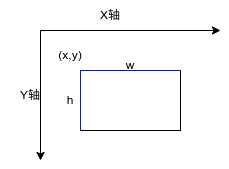
\includegraphics[width=0.3\linewidth]{box.png}
    \end{figure}
\end{frame}

\begin{frame}
    \noindent\large\textbf{基础知识}
    \begin{itemize}
        \item[$ \bullet $] 矩形框的3种表示
            矩形框的表示形式有:\\
            $[x,y,w,h]$ \\
            $[x_1,y_1,x_2,y_2]([left,top,right,bottom])$\\
            $[cx,cy,w,h]$
        \item[$ \bullet $] 交并比(IoU)
            交并比是指两个矩形的交集与并集的面积之比$IoU=\frac{|A\cap B|}{|A\cup B|}$,
            实现是采用第二种矩形表示进行实现$A[l_A,t_A,r_A,b_A],B[l_B,t_B,r_B,b_B]$:\\

            $S_A=(r_A-l_A)\times(b_A-t_A)$\\
            $S_B=(r_B-l_B)\times(b_B-t_B)$\\
            $W_{AB}=(min(r_A,r_B)-max(l_A,l_B))$\\
            $H_{AB}=(min(b_A,b_B)-max(t_A,t_B))$\\
            if $ W_{AB}<0$ or $H_{AB}<0$ then $IoU = 0$\\
            else $IoU=\frac{W_{AB}\times H_{AB}}{S_A+S_B-W_{AB}\times H_{AB}}$

    \end{itemize}
\end{frame}


\begin{frame}
    \noindent\large\textbf{常见数据集}

    %    \begin{itemize}
    %    \item[$ \bullet $]  包含图像和标签(掩码、mask、Ground Truth)
    %
    %    %\vspace{1em}
    %    \item[$ \bullet $]  图像与标签大小相同
    %
    %    %\vspace{1em}
    %    \item[$ \bullet $]  图像与标签的像素一一对应
    %
    %    %\vspace{1em}
    %    \item[$ \bullet $] 标签的形式多种多样,包括图像、描述文件、表格等形式
    %    \end{itemize}
    %
    %    \vspace{1em}
    %    \noindent\large\textbf{常见数据集}

    \vspace{1em} \small
    Common Objects in COntext(COCO)、PASCAL Visual Object Classes(PASAL)、
    The Cityscapes Dataset、The Cambridge-driving Labeled Video Database(CamVid)、
    Stanford Background Dataset、Barcelona Dataset、Microsoft Research in Cambridge、
    LITS Liver Tumor Segmentation Dataset、ISBI Challenge
\end{frame}



\begin{frame}
    \noindent\large\textbf{常用评价指标}

    \vspace{0.1em}
    $\bullet$ 准确率:$PA=\frac{TP+TN}{TP+FP+FN+TN}$

    \vspace{0.1em}
    $\bullet$ Dice系数(Dice score, F1分数):$dice(A,B)=\frac{2|A\cap B|}{|A|+|B|}=\frac{2TP}{2TP+FN+FP}$

    \vspace{0.1em}
    $\bullet$ 雅卡尔指数(交并比):$IoU=\frac{|A\cap B|}{|A \cup B|} = \frac{TP}{TP + FN + FP}$

    \vspace{0.1em}
    $IoU= \frac{Dice}{2-Dice}$; A: 目标像素的集合;B: 算法判定为目标像素的集合。除此之外还有精确率、召回率、平均准确率、平均精确率、平均召回率和聚合雅卡尔指数等指标

    \begin{figure}
        \subfloat[TP、FP、FN]{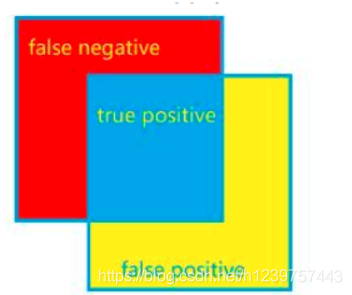
\includegraphics[width=0.3\linewidth]{TPFPFN.png}}
        \subfloat[IoU与Dice]{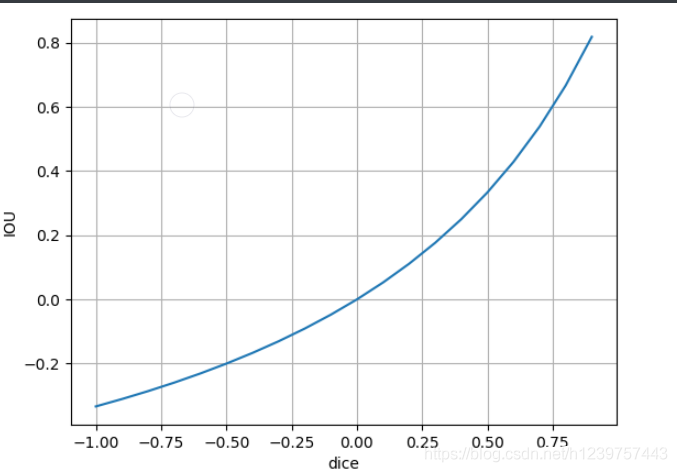
\includegraphics[width=0.3\linewidth]{IoUDice.png}}
    \end{figure}

\end{frame}

\begin{frame}
    \noindent\large\textbf{类别不平衡问题}

    \vspace{1em}
    图像当中的背景与前景常存在像素点数量不平衡的问题,这容易导致模型将所有像素点预测为同一个类别
    \begin{figure}
        
\includegraphics[width=8.0cm]{11.png}
    \end{figure}
\end{frame}

\begin{frame}
    \noindent\large\textbf{解决方法}

    \vspace{1em}
    $\bullet$ 损失函数加权:$L=\sum w_iloss_i$

    \vspace{1em}
    $\bullet$ 欠采样:样本多的类别只统计一部分像素点的损失

    \vspace{1em}
    $\bullet$ Dice损失函数:$L=1-\frac{2\sum \hat{y}_iy_i+\epsilon}{\sum (\hat{y}_i+y_i)+\epsilon}$

    \vspace{1em}
    $\bullet$ Focal损失函数:$L=-\sum (1-\hat{y}_i)^\gamma log(\hat{y}_i)$


\end{frame}

\begin{frame}
    \noindent\large\textbf{图像分割的应用}

    \vspace{1em}
    $\bullet$ 自动驾驶:对周围环境图像进行分割

    \vspace{1em}
    $\bullet$ 医学图像病灶检测:将医学影像当中的病变部位分割出来

    \vspace{1em}
    $\bullet$ 零售图像识别:对货架商品进行监控

    \vspace{1em}
    $\bullet$ 人脸识别:从图像当中提取人脸区域
\end{frame}


\section{U-net:模型与原理}
\begin{frame}[allowframebreaks]
  \frametitle{\textsc{目录}} \vspace{-0.3cm}
    \begin{spacing}{0.0}
        \tableofcontents[currentsection,hideallsubsections]
    \end{spacing}   % 若不想要目录, 注释掉该句
\end{frame}



\begin{frame}
    \noindent\large\textbf{U-net}

    \vspace{1em}
    U-net首次提出是在2015年的MICCAI会议上,此后成为了图像分割任务的baseline,
    主流的图像分割模型大多遵循U-net的基本框架。

    \begin{figure}
        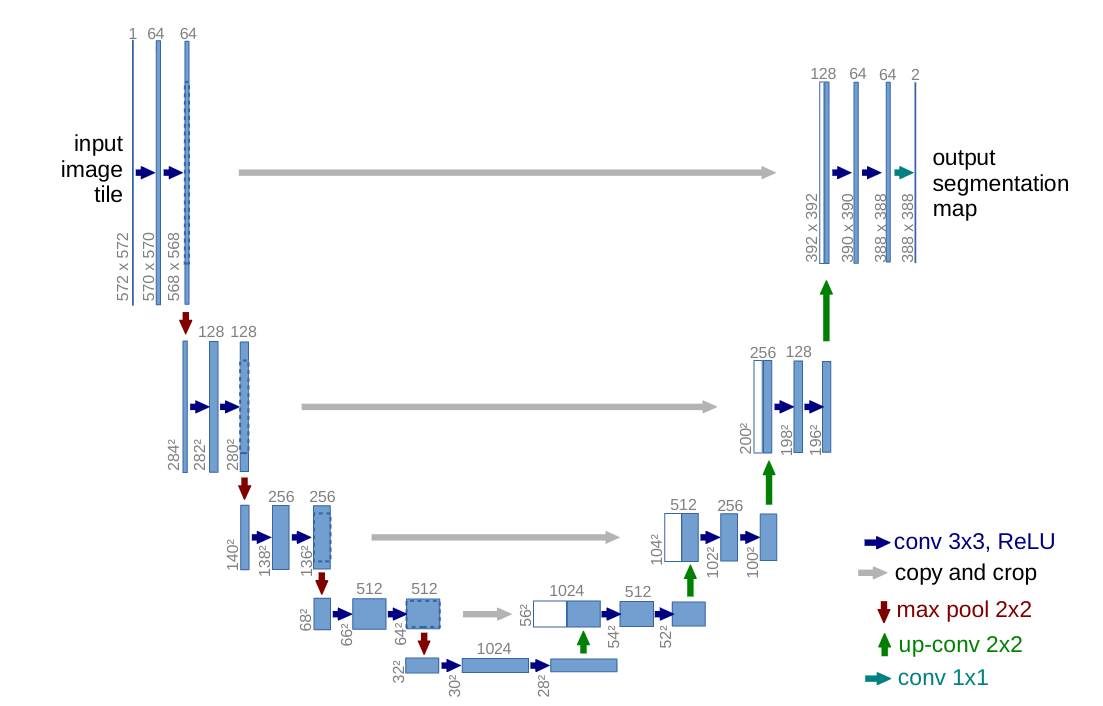
\includegraphics[width=9.5cm]{6.png}
    \end{figure}
\end{frame}

\begin{frame}
    \noindent\large\textbf{无缝分割策略}

    \vspace{1em}
    %U-net首次提出是在2015年的MICCAI会议上,此后成为了图像分割任务的baseline,
    %主流的图像分割模型大多遵循U-net的基本框架。

    \begin{figure}
        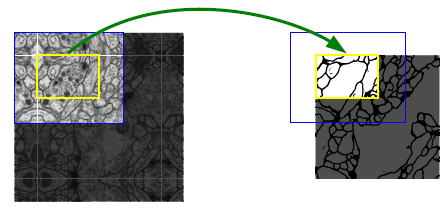
\includegraphics[width=9.5cm]{overlapTile.png}
    \end{figure}
\end{frame}

\begin{frame}
    \noindent\large\textbf{处理流程}

    \vspace{1em}
    \begin{figure}
        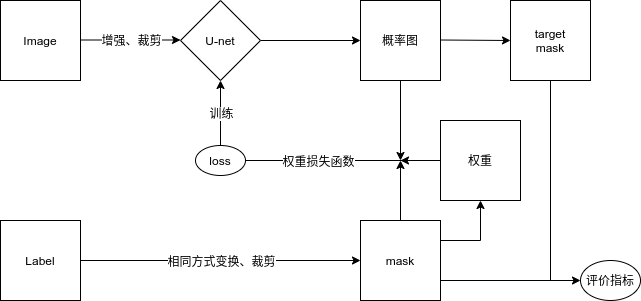
\includegraphics[width=10cm]{10.png}
    \end{figure}
\end{frame}

\begin{frame}
    \noindent\large\textbf{U-net为什么有效}

    \vspace{1em}
    $\bullet$ 跳跃连接保留了更多细节

    \vspace{1em}
    $\bullet$ 多层次特征图能够学习语义特征

    \vspace{1em}
    $\bullet$ 多层次特征融合既能保留细节又能学习语义

    \begin{figure}
        \centering
        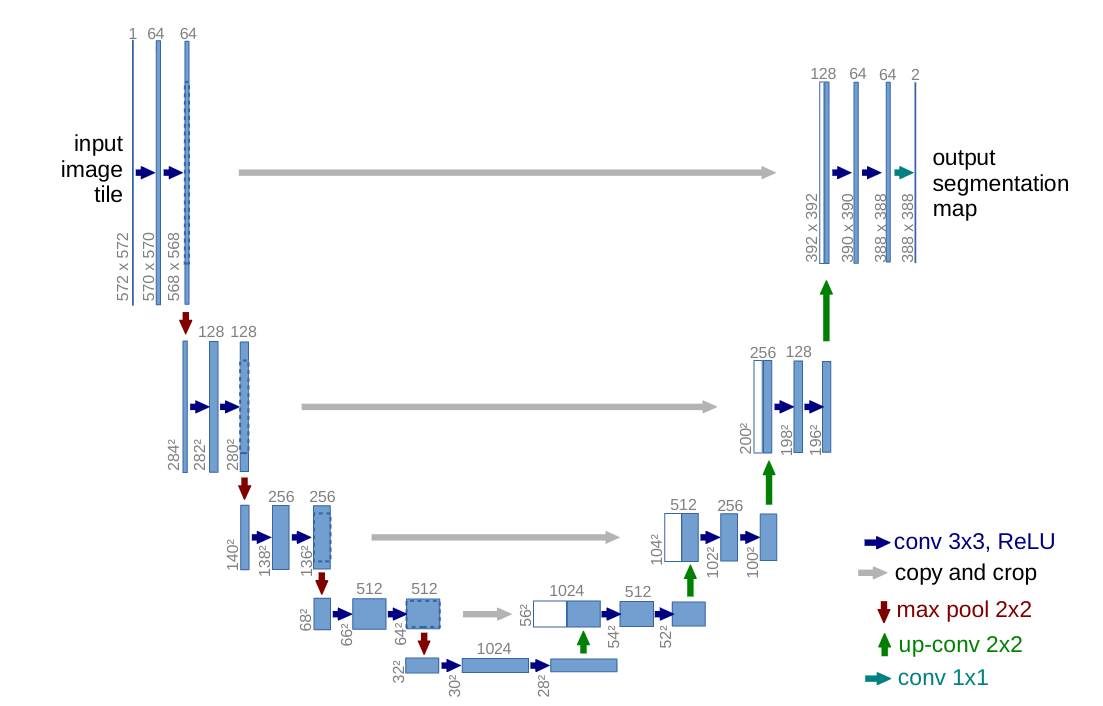
\includegraphics[height=5cm]{6.png}
    \end{figure}


\end{frame}

\begin{frame}
    \noindent\large\textbf{上采样方法}
    \vspace{1em}

    $\bullet$ 采样(线性插值、三次插值、最临近等)

    \begin{figure}
        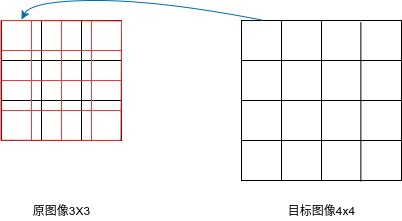
\includegraphics[width=8cm]{8.png}
    \end{figure}

    $\bullet$ 转置卷积(反卷积)
    \begin{figure}
        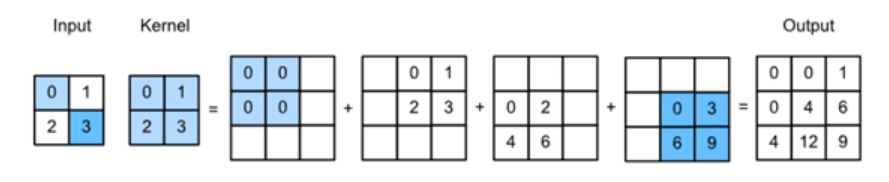
\includegraphics[width=11cm]{7.png}
    \end{figure}

\end{frame}

\begin{frame}
    $\bullet$ 上池化

    \begin{figure}
        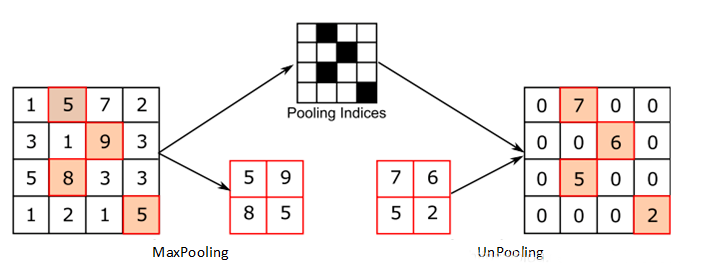
\includegraphics[width=11cm]{9.png}
    \end{figure}

    \vspace{1em}
    在pytorch的MaxPool操作当中,可以选择输出选取的位置,
    而MaxUnPool操作需要特征图和位置作为输入
\end{frame}

\begin{frame}[fragile]
    \begin{lstlisting}
# 采样
torch.nn.functional.interpolate()
torch.nn.functional.grid_sample()
torch.nn.functional.upsample()
torch.nn.UpsamplingBilinear2d
torch.nn.UpsamplingNearest2d
torch.nn.Upsample
# 转置卷积(反卷积)
torch.nn.ConvTranspose2d
torch.nn.functional.conv_transpose2d()
# 上池化
torch.nn.MaxUnpool2d
torch.nn.functional.max_unpool2d()
    \end{lstlisting}
\end{frame}

\begin{frame}

    \vspace{-5em}
    \noindent\large\textbf{特征图融合方法}


    \normalsize
    \vspace{1em}
    $\bullet$ 拼接:在通道维度上将特征图拼接起来

    \vspace{1em}
    $\bullet$ 相加:把相同形状的特征图直接相加

    \vspace{1em}
    区别:拼接不需要通道数一致但需要图尺寸相同,而相加需\\
    \quad \quad \quad 要通道数和图尺寸保持一致

    \vspace{1em}
    联系:相加可以看作是特殊的拼接,因为通常在拼接后会使用\\
    \quad \quad \quad$1\times1$卷积进行加权

\end{frame}

\begin{frame}
    \noindent\large\textbf{特征图融合方法}

    \vspace{1em}
    U-net首次提出是在2015年的MICCAI会议上,此后成为了图像分割任务的baseline,
    主流的图像分割模型大多遵循U-net的基本框架。

    \begin{figure}
        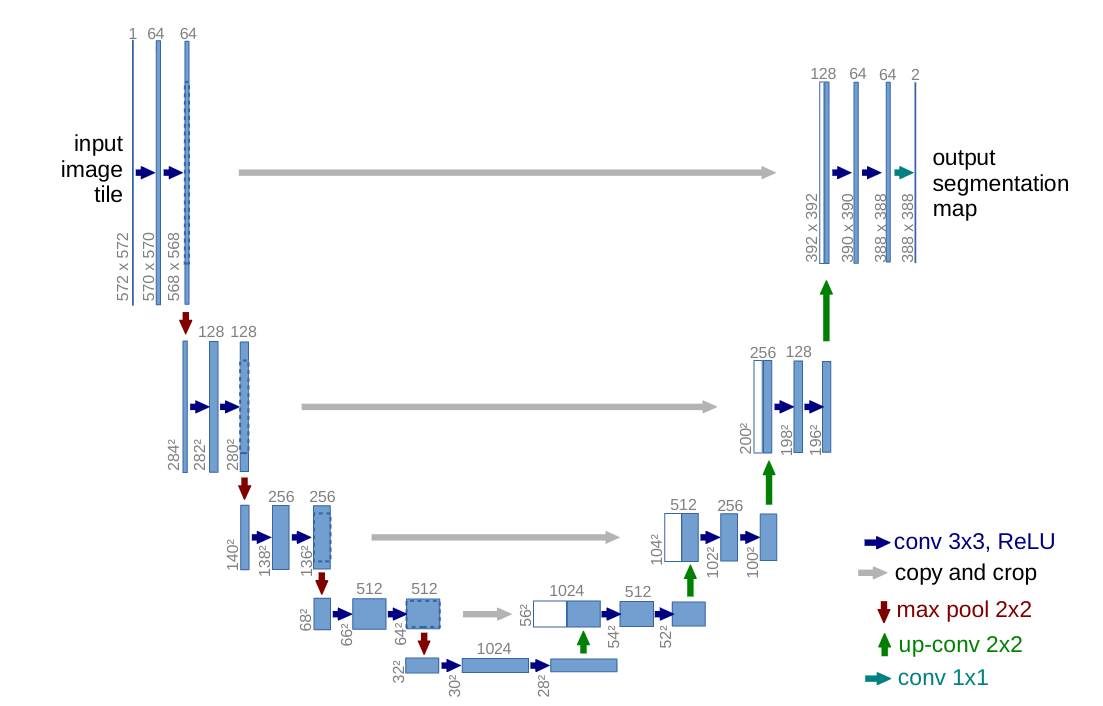
\includegraphics[width=9.5cm]{6.png}
    \end{figure}
\end{frame}


\section{目标检测方法}

\begin{frame}[allowframebreaks]
    \frametitle{\textsc{目录}} \vspace{-0.3cm}
    \begin{spacing}{0.0}
        \tableofcontents[currentsection,hideallsubsections]
    \end{spacing}   % 若不想要目录, 注释掉该句
\end{frame}

\begin{frame}
    目标检测有两个主要流派:Anchor-based与Anchor-Free,两类算法的主要区别在于算法当中是否有预设锚框\\
    \begin{itemize}
        \item[$ \bullet $] Anchor-based:YOLOv3、SSD、Faster \;R-CNN
        \item[$ \bullet $] Anchor-Free:YOLOv1、CornerNet、CenterNet、FCOS
    \end{itemize}

    \vspace{1em}
    另外一个划分是:一阶段和二阶段算法,阶段主要是指从输入到结果之间网络模型的运算次数\\
    \begin{itemize}
        \item[$ \bullet $] 一阶段:YOLO、SSD、CornerNet、CenterNet、FCOS
        \item[$ \bullet $] 二阶段:R-CNN、Faster \;R-CNN
    \end{itemize}

    \vspace{1em}
    在后面的算法当中将介绍二阶段Anchor-based算法Faster\; R-CNN和一阶段Anchor-Free算法YOLOv1\\

\end{frame}


\begin{frame}
    \noindent\large\textbf{基础知识}
    \begin{itemize}
        \item[$ \bullet $] 矩形框的3种表示
            矩形框的表示形式有:\\
            $[x,y,w,h]$ \\
            $[x_1,y_1,x_2,y_2]([left,top,right,bottom])$\\
            $[cx,cy,w,h]$
        \item[$ \bullet $] 交并比(IoU)
            交并比是指两个矩形的交集与并集的面积之比$IoU=\frac{|A\cap B|}{|A\cup B|}$,
            实现是采用第二种矩形表示进行实现$A[l_A,t_A,r_A,b_A],B[l_B,t_B,r_B,b_B]$:\\
            $S_A=(r_A-l_A)\times(b_A-t_A)$\\
            $S_B=(r_B-l_B)\times(b_B-t_B)$\\
            $W_{AB}=(min(r_A,r_B)-max(l_A,l_B))$\\
            $H_{AB}=(min(b_A,b_B)-max(t_A,t_B))$\\
            if $ W_{AB}<0$ or $H_{AB}<0$ then $IoU = 0$\\
            else $IoU=\frac{W_{AB}\times H_{AB}}{S_A+S_B-W_{AB}\times H_{AB}}$
            % \hspace{10cm}
            \vspace{-3.5cm}
            \begin{figure}
                \hspace{6cm}
                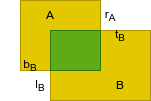
\includegraphics[width=0.4\linewidth]{iou.png}
            \end{figure}
    \end{itemize}
\end{frame}

% \begin{frame}
%     \large
%     \textcolor{vscodedef}{def}  \textcolor{vscodefuncation}{boxIou}\textcolor{vscodebracket}{(}\textcolor{vscodeparameter}{boxes1}: \textcolor{vscodeclass}{Tensor}, \textcolor{vscodeparameter}{boxes2}: \textcolor{vscodeclass}{Tensor}\textcolor{vscodebracket}{)}->\textcolor{vscodeclass}{Tensor}:\\
%     \vspace{0.2em}
%     \qquad\textcolor{vscodecomment}{\# boxes1:(N,4) boxes2:(M,4) use 'xyxy'}\\
%     \vspace{0.2em}
%     \qquad\textcolor{vscodeparameter}{area1}=\textcolor{vscodebracket}{(}\textcolor{vscodeparameter}{boxes1}\textcolor{vscodecomment}{[}:,\textcolor{vscodecomment}{2]}-\textcolor{vscodeparameter}{boxes1}\textcolor{vscodecomment}{[}:,\textcolor{vscodecomment}{0]}\textcolor{vscodebracket}{)}*\textcolor{vscodebracket}{(}\textcolor{vscodeparameter}{boxes1}\textcolor{vscodecomment}{[}:,\textcolor{vscodecomment}{3]}-\textcolor{vscodeparameter}{boxes1}\textcolor{vscodecomment}{[}:,\textcolor{vscodecomment}{1]}\textcolor{vscodebracket}{)}\\
%     \vspace{0.2em}
%     \qquad\textcolor{vscodeparameter}{area2}=\textcolor{vscodebracket}{(}\textcolor{vscodeparameter}{boxes1}\textcolor{vscodecomment}{[}:,\textcolor{vscodecomment}{2]}-\textcolor{vscodeparameter}{boxes2}\textcolor{vscodecomment}{[}:,\textcolor{vscodecomment}{0]}\textcolor{vscodebracket}{)}*\textcolor{vscodebracket}{(}\textcolor{vscodeparameter}{boxes1}\textcolor{vscodecomment}{[}:,\textcolor{vscodecomment}{3]}-\textcolor{vscodeparameter}{boxes2}\textcolor{vscodecomment}{[}:,\textcolor{vscodecomment}{1]}\textcolor{vscodebracket}{)}\\
%     \vspace{0.2em}
%     \qquad\textcolor{vscodeparameter}{lt}=\textcolor{vscodeclass}{torch}.\textcolor{vscodefuncation}{max}\textcolor{vscodebracket}{(}\textcolor{vscodeparameter}{boxes1}\textcolor{vscodecomment}{[}:,\textcolor{vscodedef}{None},:\textcolor{vscodecomment}{2]},\textcolor{vscodeparameter}{boxes2}\textcolor{vscodecomment}{[}:,:\textcolor{vscodecomment}{2]}\textcolor{vscodebracket}{)}  \textcolor{vscodecomment}{\# [N,M,2]}\\
%     \vspace{0.2em}
%     \qquad\textcolor{vscodeparameter}{rb}=\textcolor{vscodeclass}{torch}.\textcolor{vscodefuncation}{min}\textcolor{vscodebracket}{(}\textcolor{vscodeparameter}{boxes1}\textcolor{vscodecomment}{[}:,\textcolor{vscodedef}{None},\textcolor{vscodecomment}{2}:\textcolor{vscodecomment}{]},\textcolor{vscodeparameter}{boxes2}\textcolor{vscodecomment}{[}:,\textcolor{vscodecomment}{2}:\textcolor{vscodecomment}{]}\textcolor{vscodebracket}{)}  \textcolor{vscodecomment}{\# [N,M,2]}\\
%     \vspace{0.2em}
%     \qquad\textcolor{vscodeparameter}{wh}=\textcolor{vscodebracket}{(}\textcolor{vscodeparameter}{rb}-\textcolor{vscodeparameter}{lt}\textcolor{vscodebracket}{)}.\textcolor{vscodefuncation}{clamp}
%     \textcolor{vscodebracket}{(}\textcolor{vscodeparameter}{min}=\textcolor{vscodecomment}{0}\textcolor{vscodebracket}{)}\\
%     \vspace{0.2em}
%     \qquad\textcolor{vscodeparameter}{inter}=\textcolor{vscodeparameter}{wh}\textcolor{vscodebracket}{[}...,\textcolor{vscodecomment}{0}\textcolor{vscodebracket}{]}*\textcolor{vscodeparameter}{wh}\textcolor{vscodebracket}{[}...,\textcolor{vscodecomment}{1}\textcolor{vscodebracket}{]}  \textcolor{vscodecomment}{\# [N,M]}\\
%     \vspace{0.2em}
%     \qquad\textcolor{vscodeparameter}{union}=\textcolor{vscodeparameter}{area1}\textcolor{vscodebracket}{[}:,\textcolor{vscodedef}{None}\textcolor{vscodebracket}{]}+\textcolor{vscodeparameter}{area2}-\textcolor{vscodeparameter}{inter}\\
%     \vspace{0.2em}
%     \qquad\textcolor{vscodereturn}{return} \textcolor{vscodeparameter}{inter}/\textcolor{vscodeparameter}{union}
% \end{frame}

\begin{frame}
    \vspace{1em}
    \noindent\large\textbf{矩形框resize}\\
    \vspace{1em}
    在实际操作当中需要对输入的图像进行resize操作,但是这会导致矩形框的偏移,因此需要对矩形框进行相应变化\\
    \begin{figure}
        \subfloat[源图像]{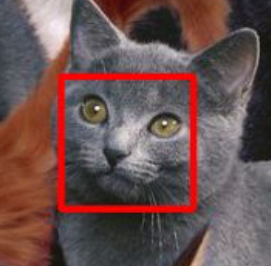
\includegraphics[width=3.3cm,height=3.3cm]{uTools_1651134324913.png}}
        \hspace{1cm}
        \subfloat[目标图像]{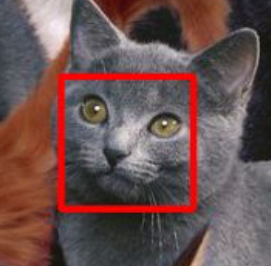
\includegraphics[width=2.4cm,height=1.5cm]{uTools_1651134324913.png}}
    \end{figure}
    图像宽高改变后,坐标点$(x,y)$和矩形框的宽高$(w,h)$按比例变化,源宽高为$(w_o,h_o)$,目标宽高为$(w_t,h_t)$:
    $$x'=\frac{xw_t}{w_o},y'=\frac{yh_t}{h_o}$$
\end{frame}

% \begin{frame}
%     \large
%     @\textcolor{vscodeclass}{no\_grad}\textcolor{vscodebracket}{()}\\
%     \vspace{0.2em}
%     \textcolor{vscodedef}{def} \textcolor{vscodefuncation}{resizeBox}\textcolor{vscodebracket}{(}\\
%     \vspace{0.2em}
%     \qquad\textcolor{vscodeparameter}{orgsize}:\textcolor{vscodeclass}{Tuple}\textcolor{vscodecomment}{[}\textcolor{vscodeclass}{int},\textcolor{vscodeclass}{int}\textcolor{vscodecomment}{]},\\
%     \vspace{0.2em}
%     \qquad\textcolor{vscodeparameter}{tarsize}:\textcolor{vscodeclass}{Tuple}\textcolor{vscodecomment}{[}\textcolor{vscodeclass}{int},\textcolor{vscodeclass}{int}\textcolor{vscodecomment}{]},\\
%     \vspace{0.2em}
%     \qquad\textcolor{vscodeparameter}{boxes}:\textcolor{vscodeclass}{Tensor}\\
%     \vspace{0.2em}
%     \qquad\textcolor{vscodebracket}{)}->\textcolor{vscodeclass}{Tensor}:\\
%     \vspace{0.2em}
%     \qquad\textcolor{vscodeparameter}{orgsize},\textcolor{vscodeparameter}{tarsize}=\textcolor{vscodeclass}{Tensor}\textcolor{vscodebracket}{(}\textcolor{vscodeparameter}{orgsize}\textcolor{vscodebracket}{)},\textcolor{vscodeclass}{Tensor}\textcolor{vscodebracket}{(}\textcolor{vscodeparameter}{tarsize}\textcolor{vscodebracket}{)}\\
%     \vspace{0.2em}
%     \qquad\textcolor{vscodeparameter}{matrix}=\textcolor{vscodeclass}{torch}.\textcolor{vscodefuncation}{diag}\textcolor{vscodebracket}{(}\textcolor{vscodeparameter}{tarsize}/\textcolor{vscodeparameter}{orgsize}\textcolor{vscodebracket}{)}\\
%     \vspace{0.2em}
%     \qquad \textcolor{vscodereturn}{return} \textcolor{vscodeclass}{torch}.\textcolor{vscodefuncation}{cat}\textcolor{vscodebracket}{(}\textcolor{vscodecomment}{[}\textcolor{vscodeparameter}{boxes}\textcolor{vscode3bracket}{[}:,:\textcolor{vscodecomment}{2}\textcolor{vscode3bracket}{]}@\textcolor{vscodeparameter}{matrix},\textcolor{vscodeparameter}{boxes}\textcolor{vscode3bracket}{[}:,:\textcolor{vscodecomment}{2}\textcolor{vscode3bracket}{]}@\textcolor{vscodeparameter}{matrix}\textcolor{vscodecomment}{]},-\textcolor{vscodecomment}{1}\textcolor{vscodebracket}{)}
% \end{frame}



\begin{frame}
    \vspace{0.5em}
    \noindent\large\textbf{非极大值抑制}\\
    \vspace{0.5em}
    非极大值抑制(NMS)主要用来去除重复的预测框,其输入是预测框数组与对应的置信度数组,算法过程如下:\\
    \vspace{0.5em}
    按置信的从大到小排序\\
    While 数组非空:\\
    \qquad 取出置信度最大的预测框 B\\
    \qquad B放入结果集\\
    \qquad 对于剩余数组当中每一个预测框b:\\
    \qquad \qquad if IoU(B,b)>阈值:\\
    \qquad \qquad \qquad 从数组中删除b\\

    \begin{figure}
        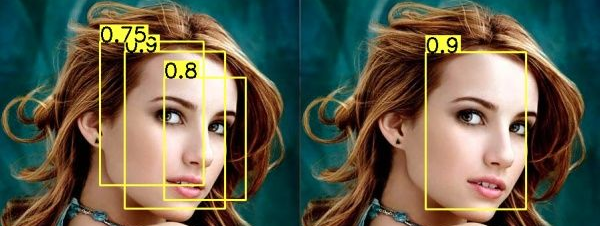
\includegraphics[width=0.7\linewidth]{NMS.png}
    \end{figure}

\end{frame}

% \begin{frame}
%     \large
%     @\textcolor{vscodeclass}{no\_grad}\textcolor{vscodebracket}{()}\\
%     \vspace{0.2em}
%     \textcolor{vscodedef}{def}  \textcolor{vscodefuncation}{nms}\textcolor{vscodebracket}{(}\textcolor{vscodeparameter}{boxes}:\textcolor{vscodeclass}{Tensor},\textcolor{vscodeparameter}{score}:\textcolor{vscodeclass}{Tensor}, \textcolor{vscodeparameter}{threshold}:\textcolor{vscodeclass}{float}\textcolor{vscodebracket}{)}->\textcolor{vscodeclass}{Tensor}:\\
%     \vspace{0.2em}
%     \qquad\textcolor{vscodecomment}{\# boxes:(N,4) score:(N)}\\
%     \vspace{0.2em}
%     \qquad\textcolor{vscodeparameter}{\_},\textcolor{vscodeparameter}{indexes}=\textcolor{vscodeparameter}{score}.\textcolor{vscodefuncation}{sort}\textcolor{vscodebracket}{(}\textcolor{vscodeparameter}{descending}=\textcolor{vscodedef}{True}\textcolor{vscodebracket}{)}\\
%     \vspace{0.2em}
%     \qquad\textcolor{vscodeparameter}{result}=\textcolor{vscodebracket}{[]}\\
%     \vspace{0.2em}
%     \qquad\textcolor{vscodereturn}{while} \textcolor{vscodecomment}{0} \textcolor{vscodedef}{not in }\textcolor{vscodeparameter}{indexes}.\textcolor{vscodeparameter}{shape}:\\
%     \vspace{0.2em}
%     \qquad\qquad\textcolor{vscodeparameter}{result}.\textcolor{vscodefuncation}{append}\textcolor{vscodebracket}{(}\textcolor{vscodeparameter}{indexes}\textcolor{vscodecomment}{[0]}\textcolor{vscodebracket}{)}\\
%     \vspace{0.2em}
%     \qquad\qquad\textcolor{vscodeparameter}{temp\_boxes}=\textcolor{vscodeparameter}{boxes}\textcolor{vscodecomment}{[}\textcolor{vscodeparameter}{indexes}\textcolor{vscodecomment}{]}\\
%     \vspace{0.2em}
%     \qquad\qquad\textcolor{vscodeparameter}{ious}=\textcolor{vscodefuncation}{boxIou}\textcolor{vscodebracket}{(}\textcolor{vscodeparameter}{temp\_boxes}\textcolor{vscodecomment}{[}:\textcolor{vscodecomment}{1]},\textcolor{vscodeparameter}{temp\_boxes}\textcolor{vscodecomment}{[1}:\textcolor{vscodecomment}{]}\textcolor{vscodebracket}{)[}\textcolor{vscodecomment}{0}\textcolor{vscodebracket}{]}\\
%     \vspace{0.2em}
%     \qquad\qquad\textcolor{vscodeparameter}{indexes}=\textcolor{vscodeparameter}{indexes}\textcolor{vscodebracket}{[}\textcolor{vscodecomment}{1}:\textcolor{vscodebracket}{][}\textcolor{vscodeparameter}{ious}<=\textcolor{vscodeparameter}{threshold}\textcolor{vscodebracket}{]}\\
%     \vspace{0.2em}
%     \qquad\textcolor{vscodereturn}{return} \textcolor{vscodeclass}{torch}.\textcolor{vscodefuncation}{stack}\textcolor{vscodebracket}{(}\textcolor{vscodeparameter}{result}\textcolor{vscodebracket}{)}
% \end{frame}
\section{Faster R-CNN}
\begin{frame}[allowframebreaks]
    \frametitle{\textsc{目录}} \vspace{-0.3cm}
    \begin{spacing}{0.0}
        \tableofcontents[currentsection,hideallsubsections]
    \end{spacing}   % 若不想要目录, 注释掉该句
\end{frame}

\begin{frame}
    \vspace{0.5em}
    \noindent\large\textbf{Faster R-CNN}\\
    \vspace{0.5em}
    Faster R-CNN是一个较为成熟的二阶段Anchor-based目标检测算法\\
    \vspace{0.5em}
    \begin{figure}
        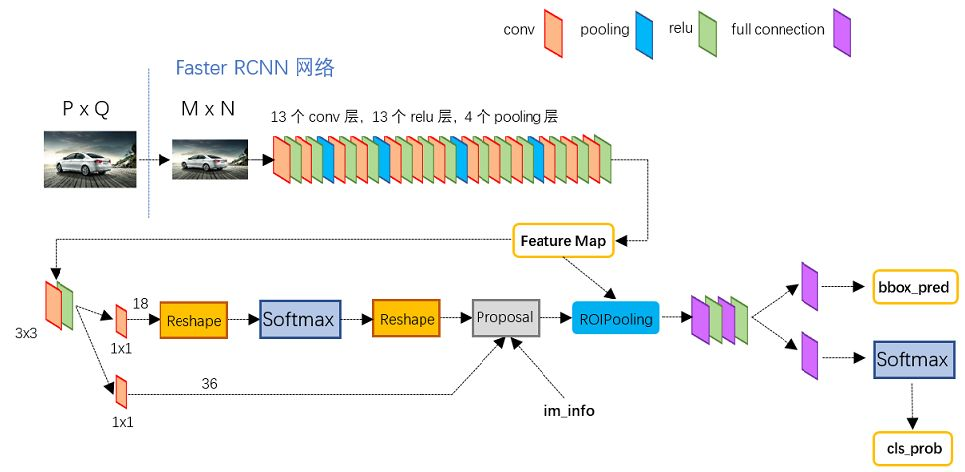
\includegraphics[width=\linewidth]{fasterrcnn.jpg}
    \end{figure}
\end{frame}

\begin{frame}
    \vspace{0.5em}
    \noindent\large\textbf{预设锚框}\\
    \vspace{0.5em}
    Faster R-CNN中设置了3种比例的锚框,1:1,1:2,2:1. 并且使用了多种尺寸,$64^2,128^2,256^2,512^2\cdots$\\
    \begin{figure}

        \subfloat{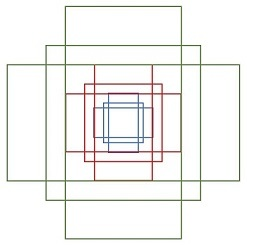
\includegraphics[width=0.3\linewidth]{anchors.jpg}}
        \hspace{0.4cm}
        \subfloat{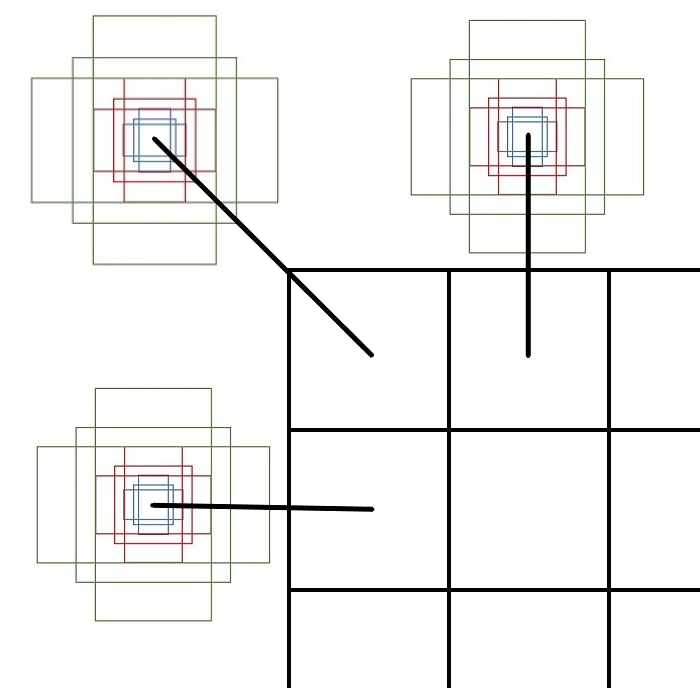
\includegraphics[width=0.3\linewidth]{anchorsposition.png}}
        \hspace{0.4cm}
        \subfloat{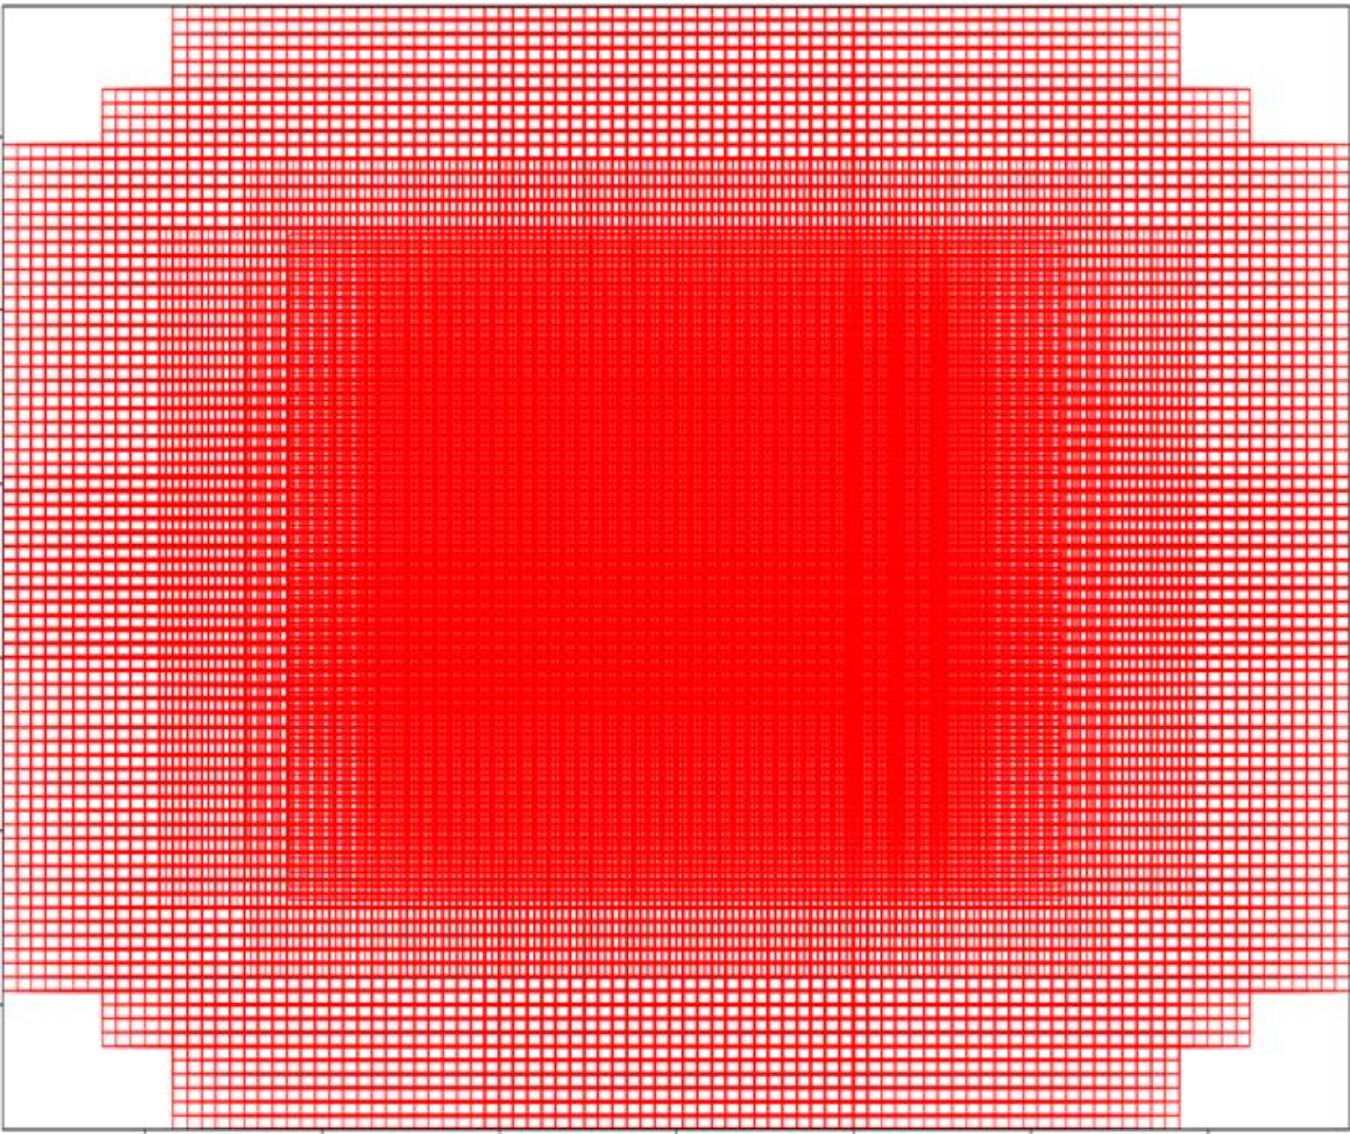
\includegraphics[width=0.3\linewidth]{uTools_1650882249335.png}}
    \end{figure}
    \vspace{0.5em}
    \noindent\large\textbf{锚框平铺}\\
    \vspace{0.5em}
    将图片分割为$P\times Q$的网格,在每一个网格上应用预设锚框,则锚框数量一共有$3\times P\times Q\times S$,其中$S$为应用的尺寸的数量.
\end{frame}
\begin{frame}
    \large
    \textcolor{vscodedef}{def}  \textcolor{vscodefuncation}{tileAnchors}\textcolor{vscodebracket}{(}\\
    \qquad\textcolor{vscodeparameter}{anchors}:\textcolor{vscodeclass}{Tensor},\\
    \qquad\textcolor{vscodeparameter}{gridsize}:\textcolor{vscodeclass}{Tuple}\textcolor{vscodecomment}{[}\textcolor{vscodeclass}{int},\textcolor{vscodeclass}{int}\textcolor{vscodecomment}{]},\\
    \qquad\textcolor{vscodeparameter}{imagesize}:\textcolor{vscodeclass}{Tuple}\textcolor{vscodecomment}{[}\textcolor{vscodeclass}{int},\textcolor{vscodeclass}{int}\textcolor{vscodecomment}{]}\\
    \qquad\textcolor{vscodebracket}{)}->\textcolor{vscodeclass}{Tensor}:\\
    \vspace{0.2em}
    \qquad\textcolor{vscodeparameter}{baselength}=\textcolor{vscodeclass}{Tensor}\textcolor{vscodebracket}{(}\textcolor{vscodeparameter}{imagesize}\textcolor{vscodebracket}{)}/\textcolor{vscodeclass}{Tensor}\textcolor{vscodebracket}{(}\textcolor{vscodeparameter}{gridsize}\textcolor{vscodebracket}{)}\\
    \vspace{0.2em}
    \qquad\textcolor{vscodeparameter}{basepos}=\textcolor{vscodeclass}{torch}.\textcolor{vscodefuncation}{stack}\textcolor{vscodebracket}{(}\textcolor{vscodeclass}{torch}.\textcolor{vscodefuncation}{meshgrid}\textcolor{vscodecomment}{(}\\
    \qquad\qquad\textcolor{vscodeclass}{torch}.\textcolor{vscodefuncation}{arange}\textcolor{vscode3bracket}{(}\textcolor{vscodeparameter}{baselength}\textcolor{vscodebracket}{[}\textcolor{vscodecomment}{0}\textcolor{vscodebracket}{]}/\textcolor{vscodecomment}{2},\textcolor{vscodeparameter}{imagesize}\textcolor{vscodebracket}{[}\textcolor{vscodecomment}{0}\textcolor{vscodebracket}{]},\textcolor{vscodeparameter}{baselength}\textcolor{vscodebracket}{[}\textcolor{vscodecomment}{1}\textcolor{vscodebracket}{]}\textcolor{vscodebracket}{)},\\
    \qquad\qquad\textcolor{vscodeclass}{torch}.\textcolor{vscodefuncation}{arange}\textcolor{vscode3bracket}{(}\textcolor{vscodeparameter}{baselength}\textcolor{vscodebracket}{[}\textcolor{vscodecomment}{1}\textcolor{vscodebracket}{]}/\textcolor{vscodecomment}{2},\textcolor{vscodeparameter}{imagesize}\textcolor{vscodebracket}{[}\textcolor{vscodecomment}{1}\textcolor{vscodebracket}{]},\textcolor{vscodeparameter}{baselength}\textcolor{vscodebracket}{[}\textcolor{vscodecomment}{1}\textcolor{vscodebracket}{]}\textcolor{vscodebracket}{)},\\
    \qquad\qquad\textcolor{vscodeparameter}{indexing}=\textcolor{vscode3bracket}{'xy'}\textcolor{vscodecomment}{)},\textcolor{vscodeparameter}{dim}=-\textcolor{vscodecomment}{1}\textcolor{vscodebracket}{)}  \textcolor{vscodecomment}{\# (H,W,2)}\\
    \vspace{0.2em}
    \qquad\textcolor{vscodeparameter}{baseanc}=\textcolor{vscodeclass}{torch}.\textcolor{vscodefuncation}{zeros}\textcolor{vscodebracket}{(}\textcolor{vscodecomment}{(}*\textcolor{vscodeparameter}{basepos}.\textcolor{vscodeparameter}{shape}\textcolor{vscode3bracket}{[}:\textcolor{vscodecomment}{2}\textcolor{vscode3bracket}{]},\textcolor{vscodeparameter}{anchors}.\textcolor{vscodeparameter}{shape}\textcolor{vscode3bracket}{[}\textcolor{vscodecomment}{0}\textcolor{vscode3bracket}{]},\textcolor{vscodecomment}{4}\textcolor{vscodecomment}{)}\textcolor{vscodebracket}{)}\\
    \vspace{0.2em}
    \qquad\textcolor{vscodeparameter}{baseanc}\textcolor{vscodebracket}{[}...,:\textcolor{vscodecomment}{2}\textcolor{vscodebracket}{]}=\textcolor{vscodeparameter}{basepos}.\textcolor{vscodefuncation}{unsqueeze}\textcolor{vscodebracket}{(}-\textcolor{vscodecomment}{2}\textcolor{vscodebracket}{)}-\textcolor{vscodeparameter}{anchors}/\textcolor{vscodecomment}{2}\\
    \vspace{0.2em}
    \qquad\textcolor{vscodeparameter}{baseanc}\textcolor{vscodebracket}{[}...,\textcolor{vscodecomment}{2}:\textcolor{vscodebracket}{]}=\textcolor{vscodeparameter}{basepos}.\textcolor{vscodefuncation}{unsqueeze}\textcolor{vscodebracket}{(}-\textcolor{vscodecomment}{2}\textcolor{vscodebracket}{)}+\textcolor{vscodeparameter}{anchors}/\textcolor{vscodecomment}{2}\\
    \vspace{0.2em}
    \qquad\textcolor{vscodereturn}{return} \textcolor{vscodeparameter}{baseanc}
\end{frame}

\begin{frame}
    \vspace{0.5em}
    \noindent\large\textbf{边框回归}\\
    \vspace{0.5em}
    在将锚框平铺到整张图像后,预设锚框基本上覆盖了所有目标,但是还不够精确,而边框回归让预测框更加准确.Faster R-CNN使用了如下形式的变换将锚框$A$映射到预测框$G$:
    \vspace{1.5em}
    \begin{flalign*}
        G_x & =A_wd_x(A)+A_x    \\
        G_y & =A_gd_y(A)+A_y    \\
        G_w & =A_wexp(d_w(A))   \\
        G_h & =A_hexp(d_h(A)) &
    \end{flalign*}
    \vspace{-4cm}
    \begin{figure}
        \hspace{4.7cm}
        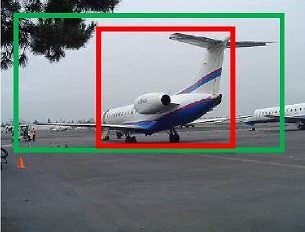
\includegraphics[width=0.4\linewidth]{reg.jpg}
    \end{figure}
    因此对预测框的校准问题就变成了对$d_x(A) d_y(A) d_w(A) d_y(A)$的回归问题

\end{frame}

\begin{frame}
    \large
    \textcolor{vscodedef}{def}  \textcolor{vscodefuncation}{calculatedxywh}\textcolor{vscodebracket}{(}\textcolor{vscodeparameter}{anchors}:\textcolor{vscodeclass}{Tensor},\textcolor{vscodeparameter}{boxes}:\textcolor{vscodeclass}{Tensor}\textcolor{vscodebracket}{)}->\textcolor{vscodeclass}{Tensor}:\\
    \vspace{0.2em}
    \qquad\textcolor{vscodecomment}{\# anchors:(...,4) boxes:(...,4)}\\

    \qquad\textcolor{vscodeparameter}{dxywh}=\textcolor{vscodeclass}{torch}.\textcolor{vscodefuncation}{zeros\_like}\textcolor{vscodebracket}{(}\textcolor{vscodeparameter}{anchors}\textcolor{vscodebracket}{)}\\

    \qquad\textcolor{vscodeparameter}{dxywh}\textcolor{vscodebracket}{[}...,:\textcolor{vscodecomment}{2}\textcolor{vscodebracket}{]}=\textcolor{vscodebracket}{(}\textcolor{vscodeparameter}{boxes}\textcolor{vscodecomment}{[}...,:\textcolor{vscodecomment}{2]}-\textcolor{vscodecomment}{anchors}\textcolor{vscodecomment}{[}...,:\textcolor{vscodecomment}{2]}\textcolor{vscodebracket}{)}/\textcolor{vscodeparameter}{anchors}\textcolor{vscodebracket}{[}...,\textcolor{vscodecomment}{2}:\textcolor{vscodebracket}{]}\\

    \qquad\textcolor{vscodeparameter}{dxywh}\textcolor{vscodebracket}{[}...,\textcolor{vscodecomment}{2}:\textcolor{vscodebracket}{]}=\textcolor{vscodeclass}{torch}.\textcolor{vscodefuncation}{log}\textcolor{vscodebracket}{(}\textcolor{vscodeparameter}{boxes}\textcolor{vscodecomment}{[}...,\textcolor{vscodecomment}{2}:\textcolor{vscodecomment}{]}/\textcolor{vscodeparameter}{anchors}\textcolor{vscodecomment}{[}...,\textcolor{vscodecomment}{2}:\textcolor{vscodecomment}{]}\textcolor{vscodebracket}{)}\\

    \qquad\textcolor{vscodeparameter}{dxywh}=\textcolor{vscodeparameter}{dxywh}.\textcolor{vscodefuncation}{nan\_to\_num}\textcolor{vscodebracket}{(}\textcolor{vscodecomment}{0}\textcolor{vscodebracket}{)}

    \qquad\textcolor{vscodereturn}{return} \textcolor{vscodeparameter}{dxywh}

    \vspace{0.5em}

    \textcolor{vscodedef}{def}  \textcolor{vscodefuncation}{applydxywh}\textcolor{vscodebracket}{(}\textcolor{vscodeparameter}{anchors}:\textcolor{vscodeclass}{Tensor},\textcolor{vscodeparameter}{dxywh}:\textcolor{vscodeclass}{Tensor}\textcolor{vscodebracket}{)}->\textcolor{vscodeclass}{Tensor}:\\

    \qquad\textcolor{vscodecomment}{\# anchors:(...,4) dxywh:(...,4)}\\

    \qquad\textcolor{vscodeparameter}{matrix}=\textcolor{vscodeclass}{torch}.\textcolor{vscodefuncation}{zeros}\textcolor{vscodebracket}{(}*\textcolor{vscodeparameter}{dxywh}.\textcolor{vscodeparameter}{shape},\textcolor{vscodecomment}{4}\textcolor{vscodebracket}{)}

    \qquad\textcolor{vscodeparameter}{matrix}\textcolor{vscodebracket}{[}...,:\textcolor{vscodecomment}{2},\textcolor{vscodecomment}{2}:\textcolor{vscodebracket}{]}=\textcolor{vscodeparameter}{dxywh}\textcolor{vscodebracket}{[}...,:\textcolor{vscodecomment}{2}\textcolor{vscodebracket}{]}.\textcolor{vscodefuncation}{diag\_embed}\textcolor{vscodebracket}{()}\\

    \qquad\textcolor{vscodeparameter}{matrix}\textcolor{vscodebracket}{[}...,:\textcolor{vscodecomment}{2},:\textcolor{vscodecomment}{2}\textcolor{vscodebracket}{]}=\textcolor{vscodecomment}{1}-\textcolor{vscodeparameter}{matrix}\textcolor{vscodebracket}{[}...,:\textcolor{vscodecomment}{2},\textcolor{vscodecomment}{2}:\textcolor{vscodebracket}{]}\\

    \qquad\textcolor{vscodeparameter}{matrix}\textcolor{vscodebracket}{[}...,\textcolor{vscodecomment}{2}:,\textcolor{vscodecomment}{2}:\textcolor{vscodebracket}{]}=\textcolor{vscodeclass}{torch}.\textcolor{vscodefuncation}{exp}\textcolor{vscodebracket}{(}\textcolor{vscodeparameter}{dxywh}\textcolor{vscodecomment}{[}...,\textcolor{vscodecomment}{2}:\textcolor{vscodebracket}{]}\textcolor{vscodebracket}{)}.\textcolor{vscodefuncation}{diag\_embed}\textcolor{vscodebracket}{()}\\

    \qquad\textcolor{vscodeparameter}{matrix}\textcolor{vscodebracket}{[}...,\textcolor{vscodecomment}{2}:,:\textcolor{vscodecomment}{2}\textcolor{vscodebracket}{]}=\textcolor{vscodecomment}{1}-\textcolor{vscodeparameter}{matrix}\textcolor{vscodebracket}{[}...,\textcolor{vscodecomment}{2}:,\textcolor{vscodecomment}{2}:\textcolor{vscodebracket}{]}\\

    \qquad\textcolor{vscodeparameter}{anchors}=\textcolor{vscodebracket}{(}\textcolor{vscodeparameter}{matrix}@\textcolor{vscodeparameter}{anchors}.\textcolor{vscodefuncation}{unsqueeze}\textcolor{vscodecomment}{(}-\textcolor{vscodecomment}{1)}\textcolor{vscodebracket}{)}.\textcolor{vscodefuncation}{squeeze}\textcolor{vscodebracket}{(}-\textcolor{vscodecomment}{1}\textcolor{vscodebracket}{)}\\

    \qquad\textcolor{vscodereturn}{return} \textcolor{vscodeparameter}{anchors}
\end{frame}

\begin{frame}
    \vspace{0.5em}
    \noindent\large\textbf{RPN层}\\
    \vspace{0.5em}
    RPN 层的主要工作是预测预设框内是否有目标物体以及预测从预设框到预测框的变换$d_{xywh}$
    \begin{figure}
        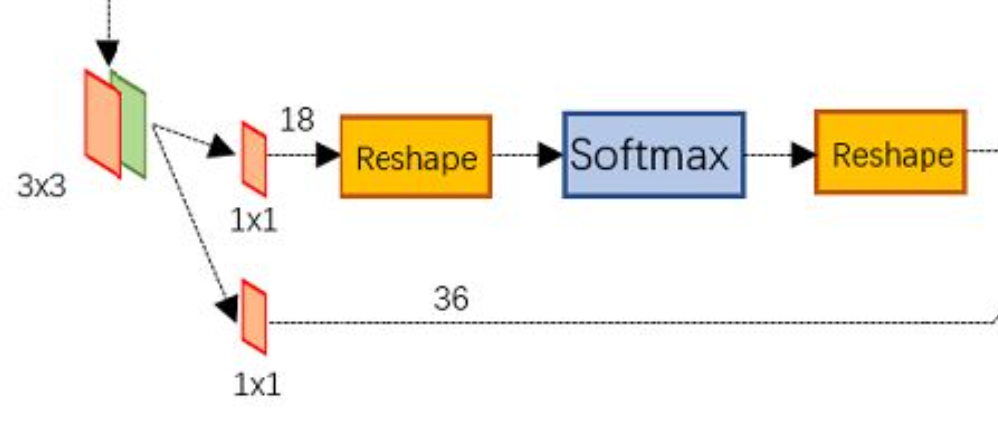
\includegraphics[width=0.8\linewidth]{RPNlayer.png}
    \end{figure}
    其中预设框内是否有目标物体是一个二分类问题,使用通道为$2K$的$1\times 1$卷积实现并且在reshape后经过Softmax运算,预测变换使用的是通道为$4K$的$1\times 1$卷积


\end{frame}

\begin{frame}
    \vspace{0.5em}
    \noindent\large\textbf{Proposal层}\\
    \vspace{0.5em}
    Proposal Layer的工作是根据RPN层的预测信息挑选出合适的预测框,算法如下:\\
    \vspace{0.2em}
    输入:预设框内有物体的置信度,预设框,变换的回归估计
    \vspace{0.2em}
    \begin{itemize}
        \item[1]根据置信度从大到小排序,选出置信度最高的N个预测框
        \item[2]使用变换的回归估计对预设框进行修正
        \item[3]修正超出图像边界的预测框
        \item[4]剔除过小的预测框
        \item[5]对剩余预测框执行非极大值抑制(NMS)
    \end{itemize}
    \vspace{0.5em}
    到这一步已经完成了"在哪里"和"有哪些"的任务,后面的工作就是分类以及对结果的轻微修正
\end{frame}

\begin{frame}
    \large
    \textcolor{vscodedef}{def}  \textcolor{vscodefuncation}{proposal}\textcolor{vscodebracket}{(}\textcolor{vscodeparameter}{anchs}:\textcolor{vscodeclass}{Tensor},\textcolor{vscodeparameter}{boxreg}:\textcolor{vscodeclass}{Tensor},\textcolor{vscodeparameter}{score}:\textcolor{vscodeclass}{Tensor},\textcolor{vscodeparameter}{N}:\textcolor{vscodeclass}{int},\\
    \qquad\textcolor{vscodeparameter}{imagesize}:\textcolor{vscodeclass}{Tuple}\textcolor{vscodecomment}{[}\textcolor{vscodeclass}{int},\textcolor{vscodeclass}{int}\textcolor{vscodecomment}{]},\textcolor{vscodeparameter}{minsize}:\textcolor{vscodeclass}{int},\textcolor{vscodeparameter}{threshold}:\textcolor{vscodeclass}{float}\textcolor{vscodebracket}{)}->\textcolor{vscodeclass}{Tensor}:\\

    \qquad\textcolor{vscodecomment}{\# anchors:(N,H,W,K,4) boxreg:(N,H,W,K,4) score:{N,H,W,K}}\\

    \qquad\textcolor{vscodeparameter}{idx}=\textcolor{vscodeparameter}{score}>\textcolor{vscodecomment}{0.5}\\

    \qquad\textcolor{vscodeparameter}{anchs},\textcolor{vscodeparameter}{boxreg},\textcolor{vscodeparameter}{score}=\textcolor{vscodefuncation}{applyIndex}\textcolor{vscodebracket}{(}\textcolor{vscodeparameter}{idx},\textcolor{vscodeparameter}{anchs},\textcolor{vscodeparameter}{boxreg},\textcolor{vscodeparameter}{score}\textcolor{vscodebracket}{)}\\

    \qquad\textcolor{vscodereturn}{if} \textcolor{vscodeparameter}{score}.\textcolor{vscodeparameter}{shape}\textcolor{vscodebracket}{[}\textcolor{vscodecomment}{0}\textcolor{vscodebracket}{]}>\textcolor{vscodeparameter}{N}:\\

    \qquad\qquad\textcolor{vscodeparameter}{idx}=\textcolor{vscodeparameter}{score}.\textcolor{vscodefuncation}{topk}\textcolor{vscodebracket}{(}\textcolor{vscodeparameter}{N}\textcolor{vscodebracket}{)}.\textcolor{vscodeparameter}{indices}\\

    \qquad\qquad\textcolor{vscodeparameter}{anchs},\textcolor{vscodeparameter}{boxreg},\textcolor{vscodeparameter}{score}=\textcolor{vscodefuncation}{applyIndex}\textcolor{vscodebracket}{(}\textcolor{vscodeparameter}{idx},\textcolor{vscodeparameter}{anchs},\textcolor{vscodeparameter}{boxreg},\textcolor{vscodeparameter}{score}\textcolor{vscodebracket}{)}

    \qquad\textcolor{vscodeparameter}{boxes}=\textcolor{vscodefuncation}{applydxywh}\textcolor{vscodebracket}{(}\textcolor{vscodeparameter}{anchors},\textcolor{vscodeparameter}{boxreg}\textcolor{vscodebracket}{)}\\

    \qquad\textcolor{vscodeparameter}{boxes}=\textcolor{vscodefuncation}{clip\_boxes\_to\_image}\textcolor{vscodebracket}{(}\textcolor{vscodeparameter}{boxes},\textcolor{vscodeparameter}{imagesize}\textcolor{vscodebracket}{)}\\

    \qquad\textcolor{vscodeparameter}{idx}=\textcolor{vscodefuncation}{remove\_small\_boxes}\textcolor{vscodebracket}{(}\textcolor{vscodeparameter}{boxes},\textcolor{vscodeparameter}{minsize}\textcolor{vscodebracket}{)}\\

    \qquad\textcolor{vscodeparameter}{boxes},\textcolor{vscodeparameter}{score}=\textcolor{vscodefuncation}{applyIndex}\textcolor{vscodebracket}{(}\textcolor{vscodeparameter}{idx},\textcolor{vscodeparameter}{boxes},\textcolor{vscodeparameter}{score}\textcolor{vscodebracket}{)}\\

    \qquad\textcolor{vscodeparameter}{idx}=\textcolor{vscodefuncation}{nms}\textcolor{vscodebracket}{(}\textcolor{vscodeparameter}{boxes},\textcolor{vscodeparameter}{minsize},\textcolor{vscodeparameter}{threshold}\textcolor{vscodebracket}{)}\\

    \qquad\textcolor{vscodereturn}{return} \textcolor{vscodeparameter}{boxes}\textcolor{vscodebracket}{[}\textcolor{vscodeparameter}{idx}\textcolor{vscodebracket}{]}.\textcolor{vscodefuncation}{clone}\textcolor{vscodebracket}{(}\textcolor{vscodebracket}{)}
\end{frame}

\begin{frame}
    \vspace{0.5em}
    \noindent\large\textbf{ROI Pooling}\\
    \vspace{0.5em}
    Region of interest pooling是对选定的区域进行采样的过程,在得到预测框后需要将区域的图像输入CNN分类器当中,这要求这些区域的分辨率保持一致.\\
    
    首先,Faster R-CNN是在下采样的特征图上进行采样的,就需要把预测框转换为特征图的尺寸.\\

    接下来,对预测框进行取整来对特征图进行切片.

    将特征图切片进行池化
\end{frame}




% \section{Reference}

% \begin{frame}[allowframebreaks]{参考文献}
%     \vspace{-0.3cm}
%     \scriptsize%\tiny\scriptsize\footnotesize\small\normalsize\large\Large\LARGE\huge\Huge
%     \normalem
%     \bibliographystyle{apalike}%{mnras}
%     \bibliography{example} % if your bibtex file is called example.bib
% \end{frame}


\end{document}
